\chapwithtoc{Introduction}
\label{intro}

\secwithtoc{Proteins and domains}
\label{intro:prodoms}

  Proteins are amino acid residue chains, polypeptides, that serve a variety of functions
  within living cells, including structural support and movement, interactions with cell's
  environment, and biochemical reaction catalysis~\cite{alberts2018molecular}.
  To function properly, proteins have to fold into their native conformation, and as
  demonstrated by \citet{anfinsen1961kinetics} on bovine pancreatic ribonuclease, the
  information for correct folding is contained in the amino acid sequence itself.

  Different sequences fold into different three-dimensional (3D) conformations.
  Certain local regions form secondary structures, such as $\alpha$-helices and
  $\beta$-sheets, and these locally ordered regions associate to form the whole protein,
  or in the case of some larger proteins, to form folding units~\cite{levitt1975computer}.
  \Citet{goldberg1969tertiary, levitt1975computer} define \emph{protein domains} as
  folding units that would be stable if we would cleave them from the rest of the protein
  molecule.
  Nevertheless, today's definition requires that these subassemblies also conceivably
  function in isolation, and members of the same \emph{domain family} tend to possess an
  ancient evolutionary relationship and often a similar
  function~\cite{ponting2002natural}.

  Many bioinformatical tools are available to perform domain identification within a
  protein sequence.
  The \emph{SCOP} database organizes proteins of known three-dimensional structures
  according to their evolutionary and structural relationship~\cite{murzin1995scop}.
  It classifies non-redundant protein domains and defines them on two main levels of SCOP
  classification, family and superfamily.
  The designation of proteins in SCOP has been constructed mainly
  manually~\cite{andreeva2020scop}.

  Other tools tend to implement semimanual approaches, often featuring
  \emph{profile hidden Markov Models} (HMMs), a powerful probabilistic method describing
  the sequence conservation in a family~\cite{krogh1994hidden, eddy1996hidden}.
  The \emph{Pfam} database~\cite{sonnhammer1997pfam} is such an example.
  Each protein family in Pfam consists of a seed alignment forming the basis to
  build an HMM-based profile~\cite{el2019pfam} by engaging the HMMER
  software~\cite{finn2010pfam, finn2011hmmer}.
  Another protein structure classification database utilizing HMMs to scan protein
  sequences against it is called \emph{CATH}~\cite{dawson2017cath}.
  CATH clusters proteins on four main levels, class (C), architecture (A), topology (T),
  and homologous superfamily (H)~\cite{orengo1997cath}.
  CATH, Pfam, and many more, are integrated in a general resource for protein families,
  domains, and functional sites, called InterPro~\cite{finn2017interpro}.
  The authors aim to create a non-redundant characterization, and the software package
  InterProScan provides an interface to functionally classify novel nucleotide or protein
  sequences~\cite{zdobnov2001interproscan}.
  By uniting the member databases, InterPro exploits their individual strengths, thus
  significantly contributing in the troublesome effort of automatic
  annotation~\cite{apweiler2000interpro}.

  % \citet{chothia1992one} predicted that there is a limited number of protein families
  % nature has used in evolution.
  % Later, \citet{wolf2000estimating} estimated the total to be between 4,000 and 7,000, and
  % the Pfam database seems to confirm this calculation, as it records 6,248 family entries
  % in release 32.0~\cite{el2019pfam}.

\secwithtoc{Protein kinase family}
\label{intro:pkinase}

  An example of a protein family is the \emph{protein kinase} (PK) family, labeled as
  \texttt{PF00069} is the Pfam database.
  PKs are enzymes transfering a phosphate group from a phosphate donor, usually
  adenosine triphosphate (ATP), onto an acceptor amino acid in a substrate protein.
  Autophosphorylation occurres as well.
  PKs are classified based on the acceptor amino acid specificity; the phosphorylated
  residues are typically serine, threonine, tyrosine, or histidine~\cite{hunter19911}.

  The PK family is large and diverse~\cite{hanks1988protein, hunter19911}, and, generally,
  PKs are involved in most of the signal transduction in eukaryotic cells.
  They control a variety of cellular processes, among others metabolism, cell cycle
  progression, differentiation, transcription, cell movement, communication, and
  apoptosis~\cite{kemp2003amp, matsuoka1998linkage, johnson1994sequential,
  vermeulen2003transcriptional, chen1994cell, warn1998regulation, cross2000serine}.
  As PKs function as a responsive regulatory system, it is not surprising that their
  turnover rate is rather fast, with a half-life averaging less than an
  hour~\cite{hunter1982phosphotyrosine}.
  Misproper PK activity can lead to unfavorable cell transformation and
  cancer~\cite{koivunen2006protein, caretta2011protein}, and therefore, they are a
  fascinating subject of study in molecular biology and bioinformatics.

  The 3D fold of PK domains is conserved~\cite{ung2018redefining} with common structural
  features specific to the PK family~\cite{taylor1994three}.
  The enzyme structure is bilobal.
  The smaller lobe on the N-terminus is composed of a five-stranded antiparallel
  $\beta$-sheet and one $\alpha$-helix~\cite{knighton1991crystal} called $\alpha$C, which
  takes part in the stabilization of the active
  conformation~\cite{mobitz2015abc, huse2002conformational}.
  The broadly helical larger lobe associated with the C-terminus adds up to have seven
  $\alpha$-helices and one antiparallel $\beta$-sheet placed on the surface of the cleft
  between the two lobes, where the catalytic site is
  located~\cite{knighton1991crystal, taylor1994three, azam2008activation}.
  Twelve major subdomain elements can be further recognized throughout the PK
  family~\cite{hanks1988protein, hanks19912, hanks1995eukaryotic}.

  \begin{figure}
    \centering
    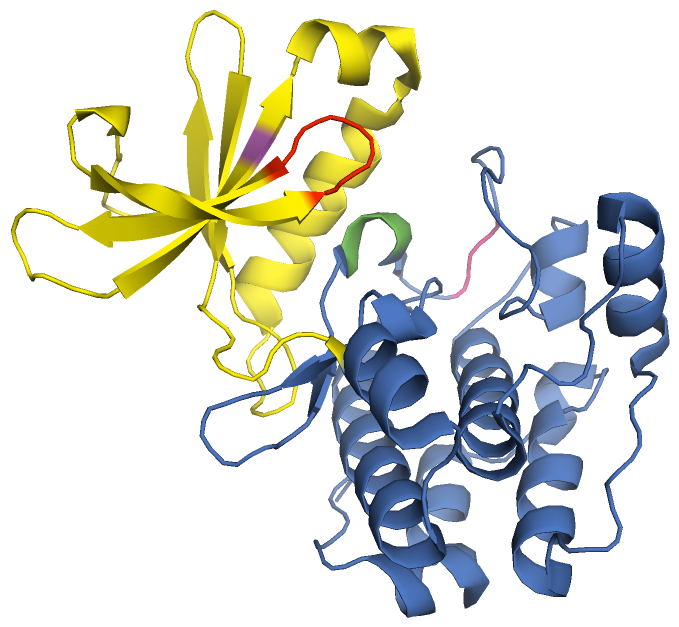
\includegraphics[width=0.8\linewidth]{img/aurora.png}
    \caption{The bilobal structure of the PK domain from the Aurora A PK.
    Structure downloaded from the PDBe, entry code 4dee~\cite{lawrence2012development},
    visualized with the PyMOL Molecular Graphics System~\cite{PyMOL}.
    Yellow: The small lobe.
    Blue: The large lobe.
    Red: Gly-X-Gly-X-X-Gly motif.
    Magenta: The invariant lysine.
    Green: DFG motif.
    Pink: APE motif.
    }
    \label{fig:aurora}
  \end{figure}

  Multiple sequence alignments (MSAs) of domains from the PK family uncover many highly
  conserved residues and motifs, some of which are strictly required for the PK activity.
  The nucleotide binding consensus sequence Gly-X-Gly-X-X-Gly is found in subdomain I and
  contains the first, second, and third essential glycine residue.
  Any side chain at the glycines' positions would interfere with the incoming ATP
  (or guanosine triphosphate (GTP)).
  The whole motif turns sharply around the nucleotide, with the first essential glycine
  being in contact with ribose, while the second provides space for the pyrophosphate
  group~\cite{wierenga1983predicted, hanks1988protein}.
  The $\beta$-phosphate moiety's oxygens are hydrogen bonded with the backbone amides of
  the residues around the third fundamental glycine, and the side chains surrounding this
  motif contribute to the hydrophobic pocket for the adenine ring of
  ATP~\cite{hanks1995eukaryotic}.
  GTP can be utilized as well, however, ATP will always have a lower Michaelis constant
  $K_{\mathrm{m}}$~\cite{hunter1985protein}.
  Regardless of which nucleotide triphosphate is used, the phosphate donor is bound as a
  complex together with a divalent cation, with $\mathrm{Mn^{2+}}$ usually preferred over
  $\mathrm{Mg^{2+}}$ and
  others~\cite{witte1980abelson, richert1979characterization, wong1984purification}.
% rozepsat PKA
  An invariant lysine in subdomain II corresponding to PKA-C$\alpha$ Lys72 is thought to
  be the best characterized catalytic domain residue~\cite{hanks1988protein}.
  It forms a salt bridge with the carboxyl group of the practically invariant glutamate in
  subdomain III, which stabilizes the interactions between the lysine and the $\alpha$-
  and $\beta$-phosphates of ATP~\cite{hanks1995eukaryotic}.
  As \citet{kamps1986neither} showed in their work on the
  p60\textsuperscript{\textit{src}} tyrosine PK, all substitutions of the lysine including
  arginine and histidine, result in a loss of the PK activity.

  A highly conserved Asp-Phe-Gly (DFG) triad can be found in subdomain VII.
  It is a part of the so-called activation loop and helps orient the $\gamma$-phosphate of
  the ATP for transfer~\cite{hanks1995eukaryotic}.
  The activation loop is centrally located and provides a platform for the peptide
  substrate by interacting with the
  $\alpha$C-helix~\cite{huse2002conformational, mobitz2015abc}.
  Autophosphorylation of certain residues within the activation loop, three tyrosines in
  case of the insulin receptor tyrosine PK, results in an active PK state; an
  unphosphorylated loop traverses through the cleft between the two lobes of the PK
  domain, thus rendering both the protein substrate and the ATP binding sites
  inaccessible~\cite{hubbard1997crystal}.
  The recognition of peptide substrates in the active state is then mediated by the
  Ala-Pro-Glu (APE) motif located in subdomain VIII~\cite{hanks1995eukaryotic}.

  Many other hydrophobic residues that do not form any primary sequence motif, or any
  particular secondary structure, characterize active PKs, as they either stabilize
  the whole domain, or regulate its overall
  activity~\cite{kornev2006surface, kornev2010defining}.
  Especially one residue called the ``gatekeeper'' lying in the hinge region between the N
  and C lobes of the PK domain has recently been of great interest in PK inhibitor
  development.
  This gatekeeper residue guards a small hydrophobic cavity neighboring the ATP-binding
  site~\cite{noble2004protein} and it anchors PK inhibitors bound in the ATP
  pocket~\cite{tong1997highly, azam2008activation}.
  The particular type of the gatekeeper residue is specific to each PK domain and the
  size and shape of the side chain determine the cavity's druggability.
  Moreover, drug design is strongly affected by the adjacent DFG motif's conformation as
  well~\cite{zuccotto2010through}.

  Still, not all members of the PK family possess the PK enzymatic
  activity~\cite{zervas2002integrin, morrison2001ksr, kroiher2001deceiving}.
  Such seemingly inactive domains may have noncatalytic functions, or do not require the
  conserved catalytic residues mentioned above and use a modified catalytic mechanism
  instead~\cite{manning2002protein}.
  However, as about two thirds of prokaryote proteins and around eighty percent of
  eukaryote proteins are multi-domain
  proteins~\cite{teichmann1998structural, gerstein1998representative}, the PK domains
  can also modulate other catalytic regions.

\secwithtoc{Multi-domain proteins}
\label{intro:multi}

  With a limited number of domain families
  present~\cite{chothia1992one, wolf2000estimating}, creating new functions may be
  somewhat difficult.
  Nature overcomes this obstacle by combining old building blocks instead of inventing new
  ones~\cite{apic2001insight}.
  \citet{muller2002structural} estimated that 98\% of the domains in the human proteome
  are duplicates; duplication is in fact one of the main sources for creation of new
  genes~\cite{lynch2000evolutionary}.
  Consequently, it is not surprising that the major molecular mechanism leading to
  multi-domain proteins and novel combination is non-homologous recombination, which is
  sometimes referred to as ``domain shuffling''~\cite{vogel2004structure}.

  Domains are not merged aimlessly when creating multi-domain proteins.
  The domain combinations seen in nature can be discriminated from a random model of
  domain combination, as shown by \citet{apic2003multi}.
  Putting together specific superfamilies results in more specific functions for
  individual molecules, and proteins with the same domain arrangement tend to be
  evolutionarily and functionally
  related~\cite{hegyi2001annotation, bashton2002geometry, vogel2004structure}.
  The sequential order of protein families identified within a protein is called
  \emph{domain architecture}.

  The set of all architectures seems to be limited as well.
  A pattern is observed, where most domains tend to have only one or few
  combination partners in the context of multi-domain proteins.
  Moreover, if a specific domain is found on the N-terminus of a particular multi-domain
  protein, other members of the same family are usually to be found on the N-terminus as
  well, and vice versa.
  The orientation and type of neighborhood varies only in a few domain families, most of
  which are large and versatile~\cite{apic2001domain, apic2001insight}.

\subsecwithtoc{Non-domain regions}
\label{intro:linker}

  Domains within the same protein are connected by non-domain amino acid stretches.
  These can be long or short, and often possess a disordered structure.
  Considering the limited number of domains and architectures in nature, these
  \emph{linkers} introduce new possibilities for structural assemblies, and may regulate,
  or sometimes even take part in the proteins' activity and
  stability~\cite{papaleo2016role}.
  Therefore, depending on the functionality of the specific domain, its associated linker
  generally requires a certain amino acid sequence~\cite{gokhale2000role}.
  It has been shown by \citet{jakubec2018widespread} that residues in pairs of domains
  coevolve, and responses to mutations in residue pairs are also observed in non-domain
  regions~\cite{smock2010interdomain}, thus ensuring a suitable environment for the whole
  molecule.

  Linkers often serve as rigid spacers between two domains.
  These molecular rulers are mostly $\alpha$-helical, and they prevent unfavorable
  interactions between the neighboring
  modules~\cite{george2002analysis, wriggers2005control}.
  Mutations in such non-domain regions are not expected to affect the function of a
  protein in any way~\cite{bottema1991missense}; in different circumstances, however,
  alterations in the linker region can have an effect on the stability, proteolytic
  resistance, or solubility of single-chain proteins~\cite{robinson1998optimizing}.
  In particular, proline is the most common residue in linkers, and careful selection of residues around prolines is of utmost importance.
  Its stiff nature helps prevent ominous contacts of linkers and domains, as it can not
  participate comfortably in any standard secondary structure conformation due to its
  inability to hydrogen bond to other
  moieties~\cite{george2002analysis, wriggers2005control}.
  Other amino acids typical for linkers are glutamine and other polar and charged
  amino acids.
  Contrarily, residues with hydrophobic or aromatic side chains are more common in
  domains~\cite{brune2018proteome}.

  Nevertheless, many linkers are also soft and intrinsically disordered.
  The non-domain region of human immunoglobulin G1 exemplifies such a flexible amino acid
  sequence~\cite{colman1976structure}.
  These often promote fundamental catalytic events in the overall function of proteins, as
  observed in the packaging of the tomato bushy stunt virus
  protein~\cite{winkler1977tomato}.
  Since soft linkers connecting domains are not merely flexible, but also allosterically
  regulated, it is no wonder that they are capable of facilitating protein folding and
  conformational changes of the whole molecule.
  The amino acid sequences of linkers, particularly of the residues in contact
  between linkers and adjoint domains, encode conformational states through which signals
  travel~\cite{george2002analysis, ma2011dynamic}.
  Examples of such signals may be the phosphorylation of a distant residue or ATP binding.
  This can be illustrated by an otherwise flexible linker in Src PKs, which clamps
  SH2 and SH3 domains upon C-terminal tyrosine phosphorylation~\cite{young2001dynamic}.
  On the other hand, ATP binding causes the immobilization of neck linkers of kinesins,
  which subsequently extend towards the plus end of a microtubule, thus giving kinesins
  their forward drive~\cite{rice1999structural, rosenfeld2001atp, khalil2008kinesin}.

  Changes in both linker length and composition can alter folding kinetics, function, and
  stability of proteins~\cite{van1997linker, robinson1998optimizing}, as demonstated in
  many studies.
  A dramatic increase of the isoelectric point (pI) from 5.86 to 9.81 was observed after a
  deletion of 40 residues from a linker in mycobacteriophage D29
  endolysin~\cite{pohane2015modulation}.
  Conformations of protein domains in cellulosomes are primarily influenced by the length
  of the linkers, as the stiffness of the linkers is inversely proportional to the linker
  length~\cite{rozycki2017length}.
  In the kinesins mentioned above, the effectivity of kinesin runs is determined by the
  length of the neck linker~\cite{shastry2010neck}.
  Domain functions are predominantly affected by short linkers, notably those that
  are buried as well.
  Contrarily, long linkers permit 3D arrangements of the domains similar to those
  accessible in multi-domain constructs with the domains swapped, hence not having so much impact on the overall protein activity~\cite{bashton2002geometry}.

  Other authors present examples where the amino acid composition is more relevant for
  the protein function compared to length.
  \citet{klement2015effect} concluded this after exploring the functionality of cytotoxic
  engineered antibody fragments.
  In addition, \citet{ikebe1998hinge} demonstrated the importance of selected linker
  residues in smooth muscle myosins, in which the actin-translocating activity was
  terminated upon deletion or substitution of these amino acids.
  As stated previously, a conserved linker sequence is crucial for the kinesins'
  microtubule-based motility as well~\cite{case2000role, hariharan2009insights}.

  Yet, it remains to be uncovered how the composition of the non-domain regions affects
  the function of multi-domain PKs in general.
  For instance, the function of PKs is regulated not only by the common structural
  elements of the PK domain, but also by the linkers~\cite{gogl2019disordered}.
  These non-core segments do not show any significant sequence similarity, and the
  composition is highly variable~\cite{taylor1994three}.
  This thesis aims to expose the relationship between the linkers' composition and PK
  activity and specificity.
  This will be done by analyzing sequences of two-domain proteins containing exactly
  one PK domain, clustering the inter-domain regions by computationally acquired
  physicochemical properties averaged over the linker sequences, and embedding unique
  \emph{Gene Ontology} (GO)~\cite{ashburner2000gene, gene2019gene} terms and \emph{Enzyme
  Commission} (EC)~\cite{webb1992enzyme, jeske2019brenda} numbers into the identified
  linker groups.
